% ============================================================
%  TERM PROJECT – PROPOSAL (template)
%  Databases · THGA Bochum
%
%  How to use:
%    1. Copy this folder into your own repository.
%    2. Replace every  <<< ... >>>  placeholder with your content.
%    3. Build with  `make`  (see the Makefile / README).
%    4. Send the resulting PDF to the lecturer and wait for approval.
% ============================================================
\documentclass[11pt,a4paper]{article}

\usepackage{thga-db}
\usepackage{caption}   % enables \captionof inside minipages

% ----- Placeholder figure (delete once you insert a real image) ----
% Draws a labelled box you can swap for \includegraphics later.
% Usage: \placeholder{width}{height}{label text}
\usetikzlibrary{positioning}
\newcommand{\placeholder}[3]{%
  \begin{tikzpicture}
    \node[draw=THGABlau!45, fill=THGABlau!5, very thick, rounded corners=2pt,
          minimum width=#1, minimum height=#2, align=center, inner sep=6pt,
          text=THGABlau!75, font=\small\itshape] {#3};
  \end{tikzpicture}%
}

% ----- Fill in your metadata -------------------------------
\renewcommand{\thgaKurs}{Databases}
\renewcommand{\thgaDatum}{Summer Term 2026}
\newcommand{\authorName}{Amen allah Dabbech}
\newcommand{\projectTitle}{Blood Donation Management System}

\begin{document}
\thispagestyle{empty}
\thgaTitel{Term Project – Proposal}{\projectTitle}

\begin{infobox}
\textbf{Author:} \authorName \\
\textbf{Module:} Introduction to Database Management Systems · THGA Bochum \\
\textbf{Submitted to:} Stephan Bökelmann · \href{mailto:sboekelmann@ep1.rub.de}{sboekelmann@ep1.rub.de} \\
\textbf{Target size:} about 6 pages
\end{infobox}

\begin{infobox}
\textbf{Every figure must be explained in the running text.} A figure never
stands on its own: refer to it by number and say what it shows -- e.g.
``Figure~\ref{fig:er} shows the ER model of \dots''. The placeholder boxes below
mark where your own images go; replace each with \texttt{\textbackslash
includegraphics} and keep the caption.
\end{infobox}

% ============================================================
\section{Application domain and motivation}
% ============================================================

Blood donation services need to continuously keep track of donors, their
donation history, and the capacity of individual donation centers. Without
digital support, it is difficult to verify whether a donor has respected the
mandatory minimum interval between two donations (e.g.\ 56 days), and centers
lack an easy overview of donor numbers and blood type distribution.

The system targets two user groups: \textbf{staff at donation centers}, who
register new donations and keep track of donors, and \textbf{administrative
staff}, who review statistics per center (e.g.\ number of donations, blood
type distribution).

\textbf{Scenario 1:} A donor arrives at a center to donate blood. Staff check
the system to see when the donor's last donation took place. If it was less
than 56 days ago, the new donation is rejected.

\textbf{Scenario 2:} An administrator wants to know how many donations a
specific center recorded last month and which blood type was most common
among them.

% ============================================================
\section{Data model -- ER sketch}
% ============================================================

\begin{figure}[ht]
  \centering
  % Replace the placeholder with: 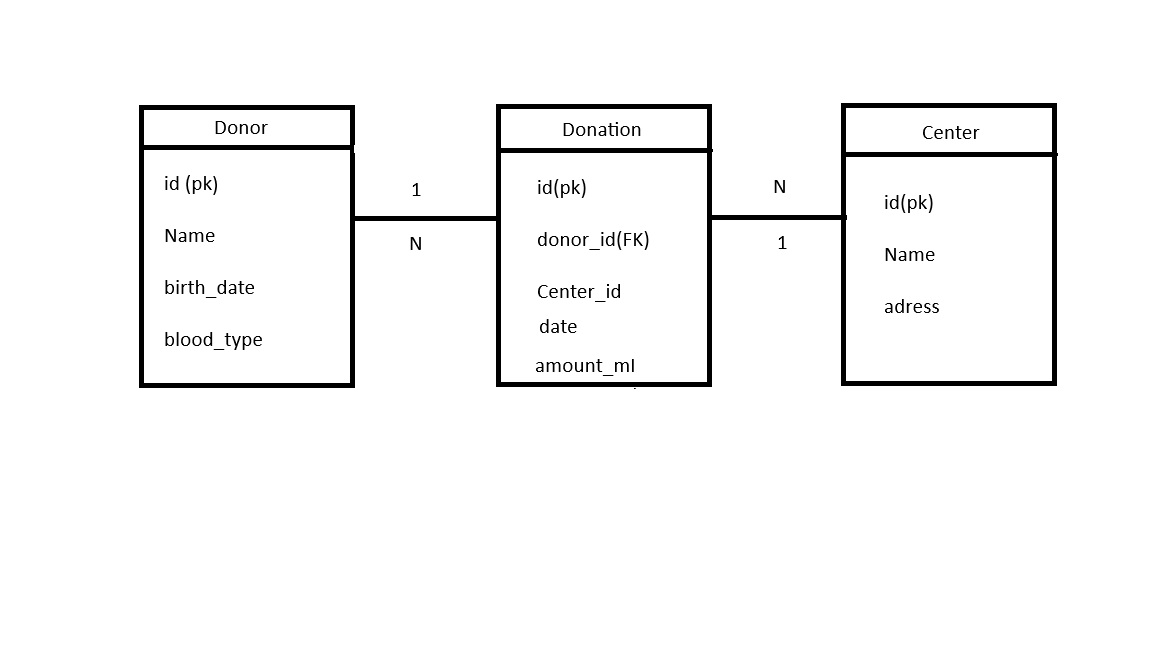
\includegraphics[width=0.85\linewidth]{er-sketch.jpg}
  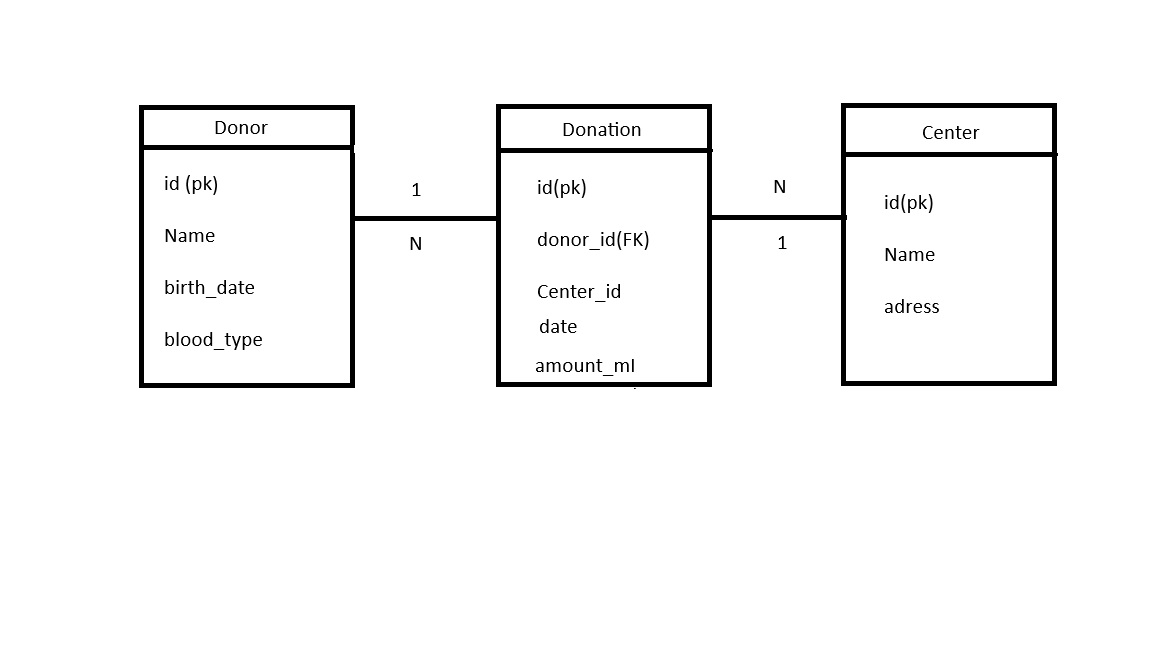
\includegraphics[width=0.85\linewidth]{er-sketch.jpeg}
  \caption{ER sketch of the blood donation data model: entity types, key
  attributes, relationships and cardinalities (at least one N:M).}
  \label{fig:er}
\end{figure}

Figure~\ref{fig:er} shows the ER model of the blood donation domain. The
central entity types are \textbf{Donor}, \textbf{Center}, and
\textbf{Donation}. Donor and Center are connected through the N:M
relationship \emph{Donation}, since one donor can donate at multiple centers
and one center serves multiple donors. Each Donation record carries its own
attributes (date, amount in ml) and links exactly one donor to exactly one
center, resulting in the cardinalities N:1 between Donation and Donor, and
N:1 between Donation and Center.

% ============================================================
\section{From model to schema}
% ============================================================

\begin{itemize}
  \item \texttt{donor(\underline{id}, name, birth\_date, blood\_type)}
  \item \texttt{center(\underline{id}, name, address)}
  \item \texttt{donation(\underline{id}, donor\_id, center\_id, date, amount\_ml)}
\end{itemize}

\textbf{Foreign keys:} \texttt{donation.donor\_id} $\rightarrow$ \texttt{donor.id};
\texttt{donation.center\_id} $\rightarrow$ \texttt{center.id}.

\textbf{Normalisation.} Each table has a single-column primary key and every
non-key attribute depends only on that key. There are no transitive
dependencies: for instance, the center's name and address are not repeated in
the \texttt{donation} table, but referenced only via \texttt{center\_id}.
Therefore the schema is in third normal form (3NF).

% ============================================================
\section{API design}
% ============================================================

\renewcommand{\arraystretch}{1.2}
\begin{tabularx}{\linewidth}{@{}p{2cm}p{4cm}X@{}}
\toprule
\textbf{Method} & \textbf{Path} & \textbf{Purpose} \\
\midrule
\texttt{GET}  & \texttt{/donors} & lists all donors \\
\texttt{GET}  & \texttt{/donors/\{id\}/donations} & donor's donation history (JOIN) \\
\texttt{GET}  & \texttt{/centers/\{id\}/stats} & donation count and total volume per center (aggregation) \\
\texttt{POST} & \texttt{/donors} & creates a new donor (requires X-API-Key) \\
\texttt{POST} & \texttt{/donations} & creates a new donation; rejected if the 56-day minimum interval is violated (requires X-API-Key) \\
\bottomrule
\end{tabularx}

% ============================================================
\section{Frontend prototype (hand sketches)}
% ============================================================

The frontend is implemented in Python using \texttt{tkinter}. It consists of
four screens: a connection dialog that collects the API URL and X-API-Key at
startup, a main screen listing all donors (calling \texttt{GET /donors}), a
detail form to register a new donation (calling \texttt{POST /donations}),
and a statistics screen showing the number of donations and total volume per
center (calling \texttt{GET /centers/\{id\}/stats}).
% The four sketches below show the four screens.
\begin{figure}[ht]
\centering
\begin{minipage}[t]{0.47\linewidth}\centering
  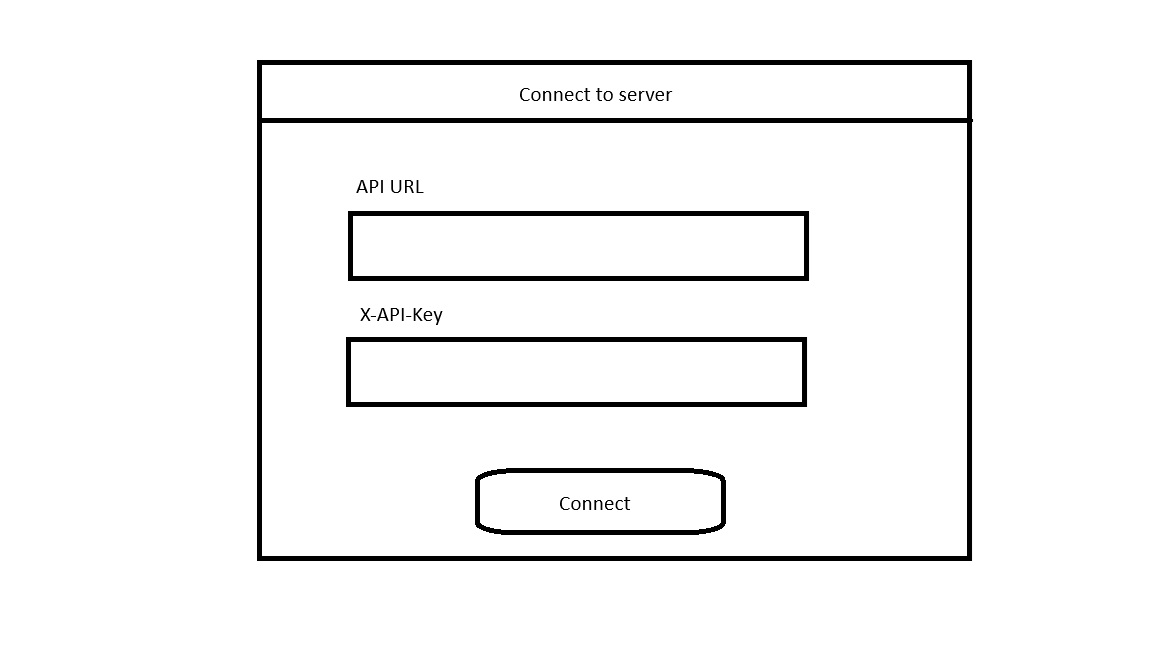
\includegraphics[width=\linewidth]{fe-connect.jpg}
  \captionof{figure}{Startup connection dialog: API URL + X-API-Key.}
  \label{fig:fe-connect}
\end{minipage}\hfill
\begin{minipage}[t]{0.47\linewidth}\centering
  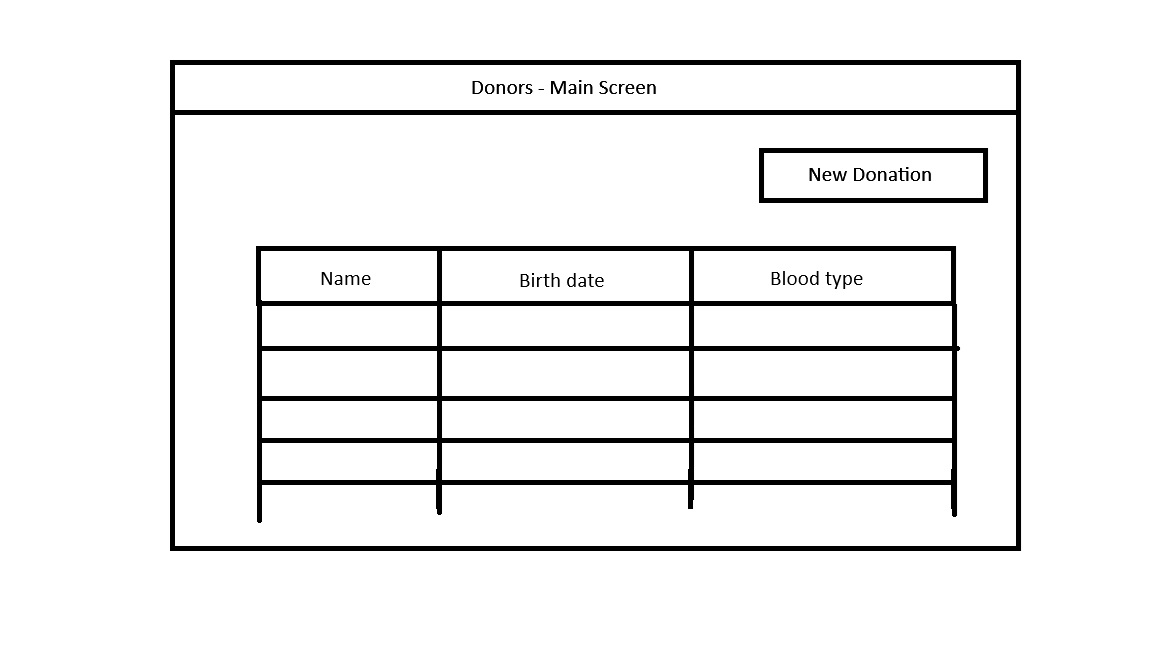
\includegraphics[width=\linewidth]{fe-main.jpg}
  \captionof{figure}{Main screen: list of all donors, calls \texttt{GET /donors}.}
  \label{fig:fe-main}
\end{minipage}
\vspace{1em}
\begin{minipage}[t]{0.47\linewidth}\centering
  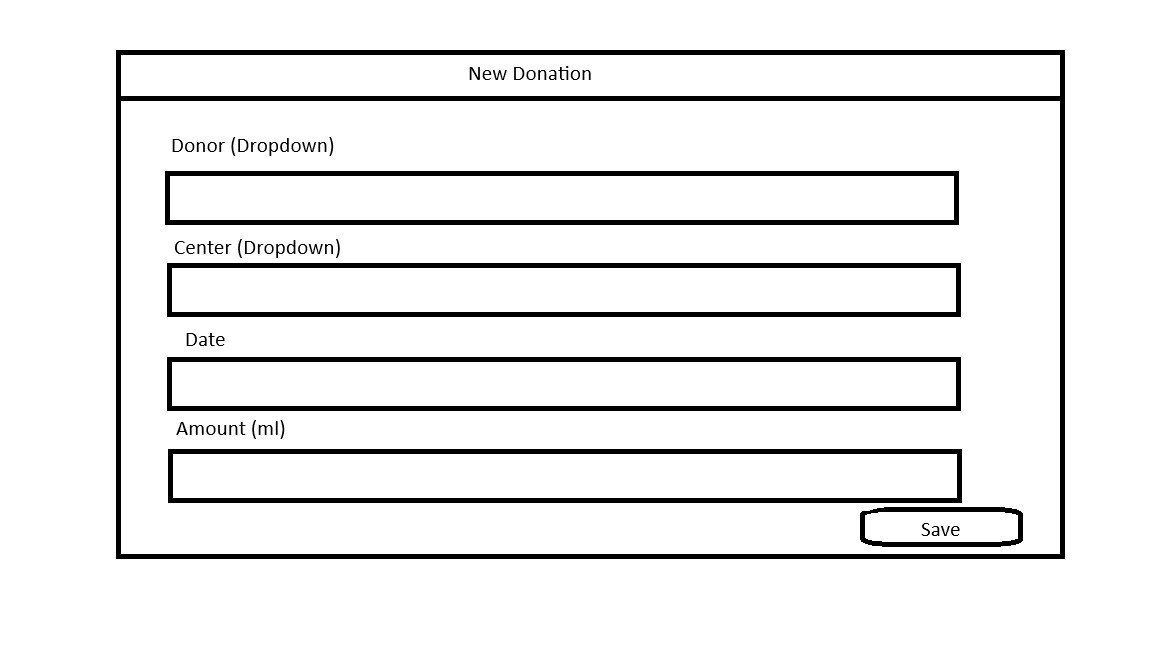
\includegraphics[width=\linewidth]{fe-detail.jpg}
  \captionof{figure}{Detail form: register a new donation, calls \texttt{POST /donations}.}
  \label{fig:fe-detail}
\end{minipage}\hfill
\begin{minipage}[t]{0.47\linewidth}\centering
  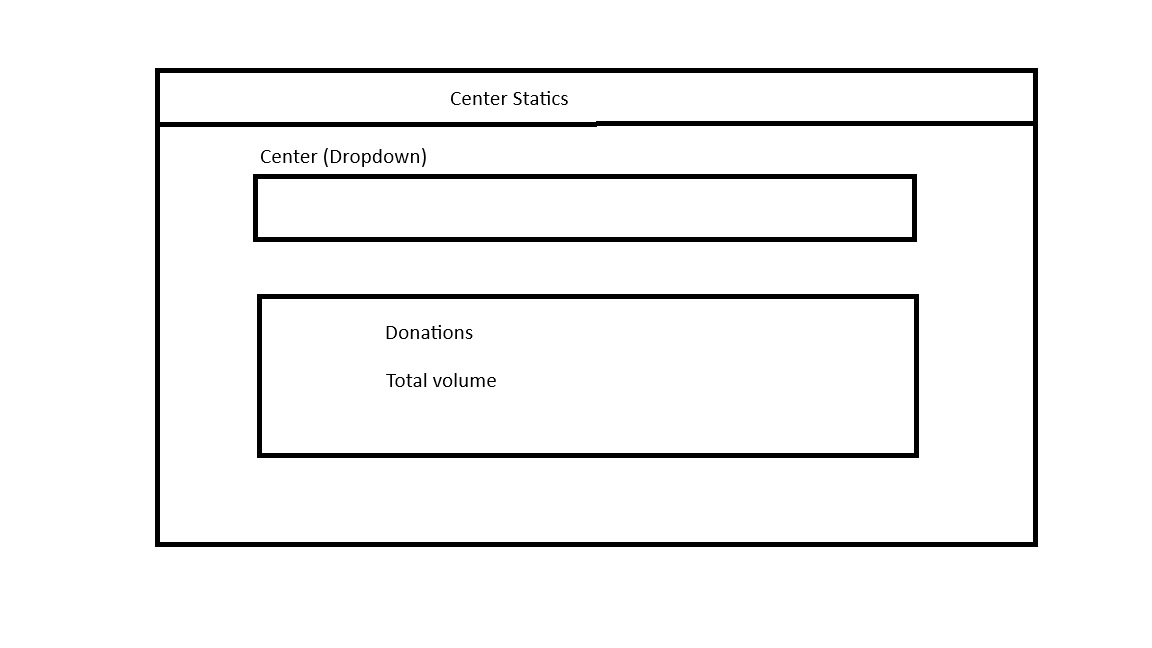
\includegraphics[width=\linewidth]{fe-second.jpg}
  \captionof{figure}{Center statistics screen, calls \texttt{GET /centers/\{id\}/stats}.}
  \label{fig:fe-second}
\end{minipage}
\end{figure}
Figures~\ref{fig:fe-connect}--\ref{fig:fe-second} show the four screens of the
prototype. Figure~\ref{fig:fe-connect} shows the connection dialog that
collects the API URL and X-API-Key at startup; Figure~\ref{fig:fe-main}
shows the main screen listing all donors, read via \texttt{GET /donors};
Figure~\ref{fig:fe-detail} shows the form used to register a new donation,
calling \texttt{POST /donations}; and Figure~\ref{fig:fe-second} shows the
center statistics screen, calling \texttt{GET /centers/\{id\}/stats}.

% ============================================================
\section{Operation with Docker Compose}
% ============================================================

The system runs via Docker Compose with two services: \texttt{postgres} (the
database) and \texttt{api} (the FastAPI backend). The \texttt{postgres}
service persists data in a named volume, so donor and donation records
survive container restarts. Database credentials and the X-API-Key are
stored in a \texttt{.env} file, which is not committed to version control and
is only read at container startup via \texttt{env\_file} in
\texttt{docker-compose.yml}. On the lecture server, the backend is deployed
by pulling the repository, placing the \texttt{.env} file, and running
\texttt{docker compose up -d}; the API is then reachable over HTTP on the
configured port, and the frontend connects to it using the API URL and
X-API-Key entered in the startup dialog.


% ============================================================
\section{Scope, milestones and risks}
% ============================================================

\textbf{Scope.} The system consists of 3 tables (\texttt{donor},
\texttt{center}, \texttt{donation}) and 5 API endpoints (3 GET, 2 POST).

\textbf{Milestones and schedule.}

\begin{center}
\renewcommand{\arraystretch}{1.2}
\begin{tabularx}{0.95\linewidth}{@{}p{1.2cm}p{8cm}p{1.8cm}@{}}
\toprule
\textbf{Week} & \textbf{Milestone} & \textbf{Est. hours} \\
\midrule
1 & Schema design and seed data ready & 8 \\
2--3 & API reading/writing implemented, protected by X-API-Key & 12 \\
4--5 & Frontend (tkinter) operates the core endpoints, packaged as .deb & 10 \\
6 & Tests, documentation, and video & 10 \\
\bottomrule
\end{tabularx}
\end{center}

\textbf{Risks.} The main risk is that the minimum-interval constraint between
two donations is not enforced correctly, allowing invalid donations to be
recorded. A second risk is that the .deb packaging of the tkinter frontend
takes longer than planned, reducing time available for testing.
% ============================================================
\section{Acceptance criteria and testing}
% ============================================================

This section states when the system counts as done and correct, and how each
claim is verified. Each criterion is formulated as a checkable statement,
backed by a concrete test; the risk from Section~7 is covered by a dedicated
test case for the minimum-interval rule.

\textbf{Acceptance criteria.}
\begin{itemize}[topsep=2pt]
  \item A donation that violates the 56-day minimum interval is rejected (API returns 4xx).
  \item \texttt{GET /centers/\{id\}/stats} returns the correct donation count and total volume (JOIN + aggregation).
  \item Write endpoints (\texttt{POST /donors}, \texttt{POST /donations}) without a valid X-API-Key are refused (401/403).
\end{itemize}

\textbf{Test plan.}
\begin{itemize}[topsep=2pt]
  \item \textbf{Database:} verify PK uniqueness on all tables, FK constraints
        between \texttt{donation} and \texttt{donor}/\texttt{center}, and
        NOT NULL constraints on required fields such as \texttt{date} and \texttt{amount\_ml}.
  \item \textbf{API:} endpoint tests covering happy path and error cases (invalid
        donor/center id, missing fields) using \texttt{pytest} and FastAPI's
        \texttt{TestClient} against a test database (L 08).
  \item \textbf{Business rule:} a test that inserts a donation less than 56 days
        after a donor's previous donation and asserts the API rejects it.
\end{itemize}
\vspace{1em}
\begin{infobox}
\textbf{Effort budget:} the whole term project (system, documentation and video)
should fit into roughly \textbf{40\,h of work} over at most \textbf{2 months}.
Keep your scope within that budget.
\end{infobox}

\end{document}
